\documentclass[tikz,border=8pt]{standalone}
% Shared look for every TikZ diagram. Load with \input{../../tools/tikz-style.tex}
\usepackage[T1]{fontenc}
\usepackage{lmodern}
\renewcommand{\sfdefault}{lmr}  % diagrams use the same serif as the text
\usetikzlibrary{arrows.meta, positioning, shapes.geometric, calc, fit, backgrounds}
\definecolor{cblue}{HTML}{4C78A8}
\definecolor{corange}{HTML}{F58518}
\definecolor{cgreen}{HTML}{54A24B}
\definecolor{cred}{HTML}{E45756}
\definecolor{cpurple}{HTML}{B279A2}
\definecolor{cgrey}{HTML}{6B6B6B}
\tikzset{
  every picture/.style={font=\sffamily, line width=1.2pt},
  box/.style={draw=#1, fill=#1!12, rounded corners=4pt, align=center, inner sep=7pt, minimum height=1.1cm},
  box/.default=cgrey,
  arrow/.style={-{Stealth[length=3mm]}, draw=cgrey, line width=1.4pt},
  title/.style={font=\sffamily\bfseries\Large},
  note/.style={font=\sffamily\small, text=cgrey, align=center},
}
\AtBeginDocument{\hyphenpenalty=10000 \exhyphenpenalty=10000}

\begin{document}
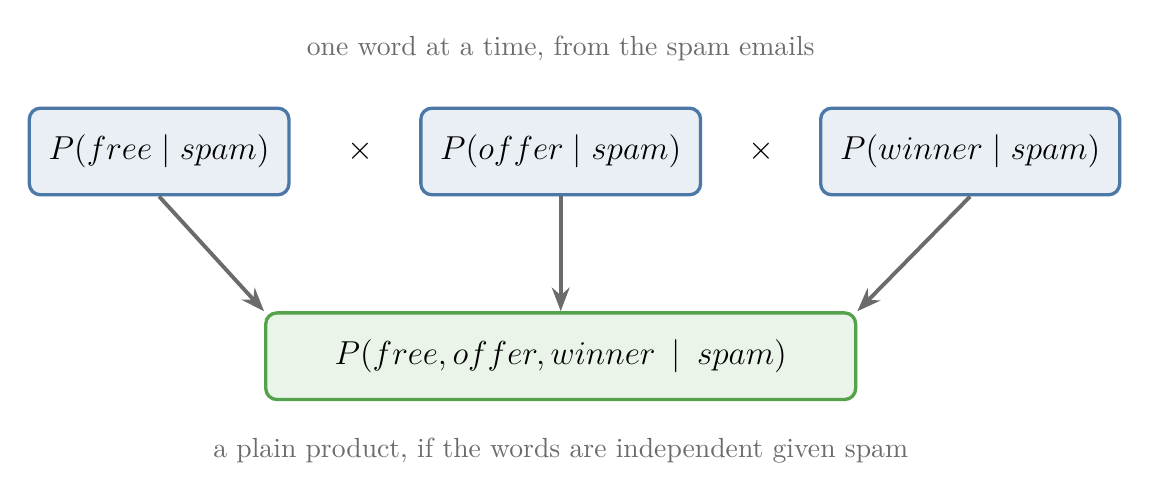
\begin{tikzpicture}[every node/.append style={font=\sffamily\large}]
  \node[box=cblue] (a) at (0,0) {$P(\text{free} \mid \text{spam})$};
  \node at (2.55,0) {$\times$};
  \node[box=cblue] (b) at (5.1,0) {$P(\text{offer} \mid \text{spam})$};
  \node at (7.65,0) {$\times$};
  \node[box=cblue] (c) at (10.3,0) {$P(\text{winner} \mid \text{spam})$};
  \node[box=cgreen, text width=7cm] (all) at (5.1,-2.6) {$P(\text{free, offer, winner} \mid \text{spam})$};
  \draw[arrow] (a.south) -- (all.north west);
  \draw[arrow] (b.south) -- (all.north);
  \draw[arrow] (c.south) -- (all.north east);
  \node[note, font=\sffamily] at (5.1,1.3) {one word at a time, from the spam emails};
  \node[note, font=\sffamily] at (5.1,-3.8) {a plain product, if the words are independent given spam};
\end{tikzpicture}
\end{document}
